\documentclass[compress]{beamer}

\usepackage[utf8]{vntex}
\usepackage{longtable}
\usepackage{amsmath}
\usepackage{amsmath}
\usepackage{amsfonts}
\usepackage{amssymb}
\usepackage[utf8]{inputenc}
\usepackage[absolute,overlay]{textpos}

\usepackage{listings}
\lstset{
	language = Java,
	frame = single,
	tabsize = 3
}

\usetheme{Warsaw}
%\usetheme{Antibes}
%\usecolortheme{spruce}
%\setbeamercolor{structure}{fg=cyan!90!blue}

\expandafter\def\expandafter\insertshorttitle\expandafter{%
    \insertshorttitle\hfill%
    \insertframenumber\,/\,\inserttotalframenumber}
      
\AtBeginSection[] % Do nothing for \section*
{
\begin{frame}
\tableofcontents[currentsection]
\end{frame}
}
\AtBeginSubsection[] % Do nothing for \section*
{
\begin{frame}
\tableofcontents[currentsection, currentsubsection]
\end{frame}
}

\author{Nguyễn Tuấn Đạt, Phan Anh Tú (SoICT-HUST)}

\begin{document}


 
\begin{frame}
\begin{center}
\huge \bf Đề tài:\\ Phân tích quan điểm
\end{center}
\vspace{0.7cm}
\textbf{Nhóm sinh viên thực hiện:}\\[0.1cm]
\begin{columns}
\column{.30\textwidth}
Phan Anh Tú\\ 
Nguyễn Tuấn Đạt 
\column{.30\textwidth} 
MSSV:20134501\\
MSSV:20130856
\column{.30\textwidth}
Lớp:CNTT2.01-K58\\
Lớp:CNTT2.02-K58
\end{columns}
\vspace{1cm}
\textbf{Giảng viên:} PGS.TS Lê Thanh Hương
\end{frame} 

\begin{frame}{Phân công công việc}
\begin{itemize}
\item Nguyễn Tuấn Đạt
\begin{itemize}
\item Tìm hiểu và cài đặt SVM
\end{itemize}
\item Phan Anh Tú
\begin{itemize}
\item Tìm hiểu và cài đặt LSTM
\end{itemize}
\end{itemize}
\end{frame}
  
   
\begin{frame}{Nội dung trình bày}
\tableofcontents
\end{frame}

\section{Giới thiệu bài toán}
\begin{frame}{Giới thiệu bài toán}
\begin{itemize}
\onslide<1->\item Input: Các câu văn.
\onslide<2->\item Output: Nhãn cho các câu văn đầu vào
\begin{itemize}
\item Hai nhãn: Tích cực, tiêu cực
\item Nhiều nhãn
\end{itemize}
\end{itemize}
\end{frame}

\section{Xử lý dữ liệu}
\begin{frame}{One-hot vector}
\begin{itemize}
\onslide<1->\item Các từ biểu bằng một vector độ dài của từ điển
\onslide<2->\item Vị trí của từ trong từ điển trong vector có giá trị 1
\end{itemize}
\onslide<3->
\begin{figure}
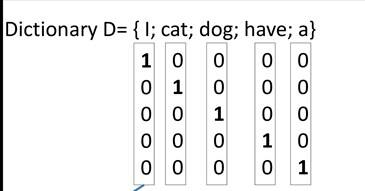
\includegraphics[scale=0.5]{one_hot_vector.jpg}
\caption{One-hot vector}
\end{figure}
\end{frame}

\begin{frame}{Continuous Bag of Words Model (CBOW)}
\only<1>{\begin{itemize}
\item Đoán các từ trung tâm dựa vào ngữ cảnh xung quanh. 
\centerline{\emph{"The cat jumped over puddle"}}
\begin{itemize}
\item C = 2 
\item context của từ \emph{"jumped"}: \{ \emph{"the", "cat", "over", "puddle"} \}.
\end{itemize}
\item Đầu vào: Tập các câu
\item Đầu ra: Embedded vector của các từ trong từ điển
\item Cần học 2 ma trận tham số $V \in \mathbb{R}^{n \times |D|}$, $U \in \mathbb{R}^{|D| \times n}$
\begin{itemize}
\item $n$ là số chiều của word vector mong muốn
\item Cột i của ma trận $V$ là embedded vector $n$ chiều của từ thứ i trong từ điển khi nó được input vào mô hình, 
\item Hàng thứ i của ma trận $U$ là embedded vector $n$ chiều của từ thứ i khi output ra khỏi mô hình.
\end{itemize}
\item $U$ là ma trận các embedded vector đầu ra
\end{itemize}}

\only<2>{\begin{itemize}
\item Tạo các one-hot vector cho các từ trong tập context ($x^{c-m}, ..., x^{c-1}, x^{c+1}, ..., x^{c+m}$)
\item Tính các embedded word vector cho mỗi context ($v_{c-m} = Vx^{x-m}, v{c-m+1} = Vx^{c-m+1}, ...., v_{c+m} = Vx^{c+m}$).
\item Tính trung bình các vector $\hat{v} = \frac{v_{c-m} + v_{c-m+1} + .... + v_{c+m}}{2m}$
\item Sinh ra vector đánh giá $z = U\hat{v}$
\item Tính vector đầu ra $\hat{y} = softmax(z)$
\item Tính lỗi của vector đầu ra so với vector của center word thực tế sử dụng hàm cross-entropy
$$H(\hat{y},y) = -\sum_{j=1}^{|V|} y_jlog(\hat{y}_j)$$
\item Update các ma trận $U, V$ để cực tiểu hóa hàm lỗi.
\end{itemize}}
\end{frame}

\begin{frame}{Skip-Gram}
\begin{itemize}
\item Dự đoán các từ xung quanh dựa vào từ trung tâm
\item Học 2 ma trận $U,V$
\begin{itemize}
\item Tạo one-hot vector cho center word $x$.
\item Tính embedded word vector cho $x$: $v_c = Vx$
\item Tính 2m vector đánh giá $u_{c-m} = u_{c-m+1} = .... = u_{c+m} = u = Uv_c$
\item Với mỗi vector $u_i$ tính vector đầu ra $y_i = softmax(u)$
\item Hàm lỗi trở thành:
$$H = \sum_{j=c-m}^{c+m} H(\hat{y}_j,y_j) \quad j \neq c$$
\item Update các ma trận $U, V$ để cực tiểu hóa hàm lỗi sử dụng chiến lược \emph{Stochastic Gradient Desecent}
\end{itemize}
\end{itemize}
\end{frame}

\section{Các phương pháp áp dụng}
\subsection{SVM}
\begin{frame}{SVM}
\end{frame}

\subsection{LSTM}
\begin{frame}{RNN}
\begin{itemize}
\onslide<1->\item Là một mô hình phổ biến trong nhiều bài toán liên quan đến xử lý ngôn ngữ tự nhiên
\onslide<2->\item Sử dụng các thông tin liên tục (ghi nhớ các thông tin đã xử lý ở quá khứ) 
\onslide<3->
\begin{figure}[H]
\centering
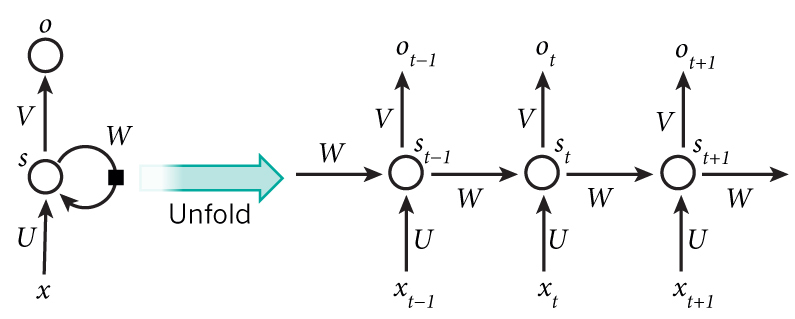
\includegraphics[scale=0.3]{rnn.jpg}
\caption{Mạng RNN}
\end{figure}
\onslide<4-> \item Vấn đề Long-Term Dependencies
\end{itemize}
\end{frame}

\begin{frame}{LSTM}
\only<1>{
\begin{textblock*}{3cm}(1cm,2.5cm)
\begin{figure}[H]
\centering
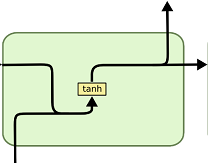
\includegraphics[scale=0.55]{rnn_tanh.png}
\caption{Một module của RNN chuẩn}
\end{figure}
\end{textblock*}

\begin{textblock*}{3cm}(7cm,2.5cm)
\begin{figure}[H]
\centering
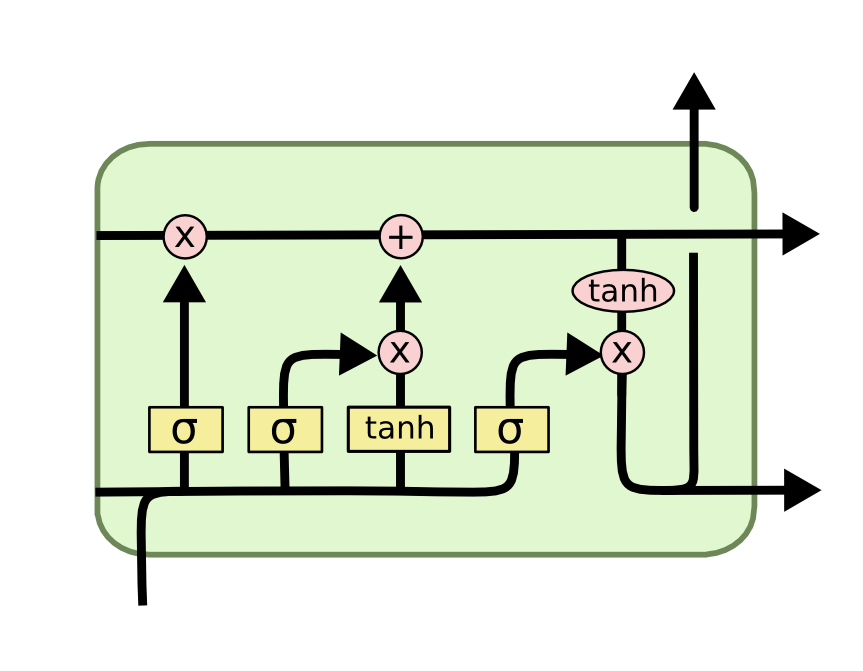
\includegraphics[scale=0.4]{lstm_module.png}
\caption{Một module của LSTM}
\end{figure}

\end{textblock*}
}
\only<2>{
\begin{figure}[H]
\centering
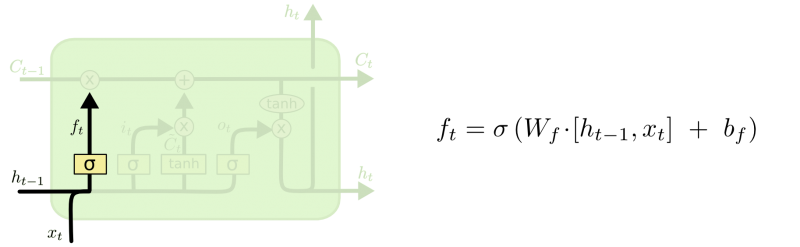
\includegraphics[scale=0.4]{lstm_module_firststep.png}
\caption{Forget gate layer}
\end{figure}
}
\only<3>{
\begin{figure}[H]
\centering
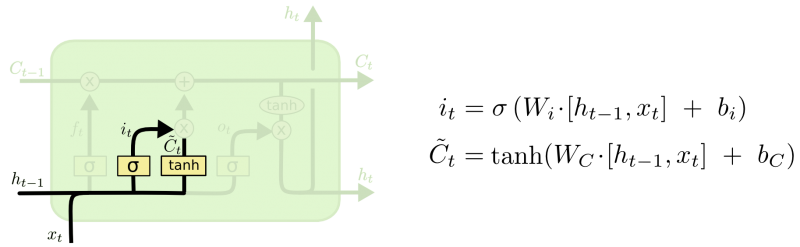
\includegraphics[scale=0.4]{lstm_module_secondstep.png}
\caption{Input gate layer}
\end{figure} 
}
\only<4>{
\begin{figure}[H]
\centering
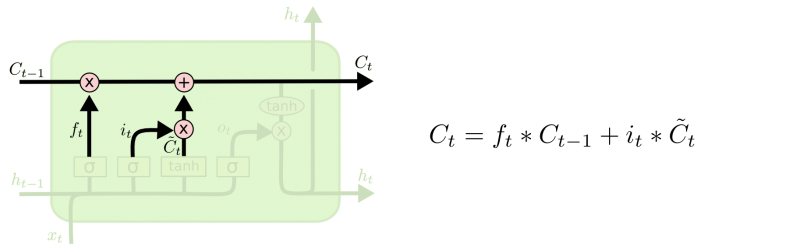
\includegraphics[scale=0.4]{lstm_module_update_cellstate.png}
\caption{Cập nhật cell state}
\end{figure} 
}
\only<5>{
\begin{figure}[H]
\centering
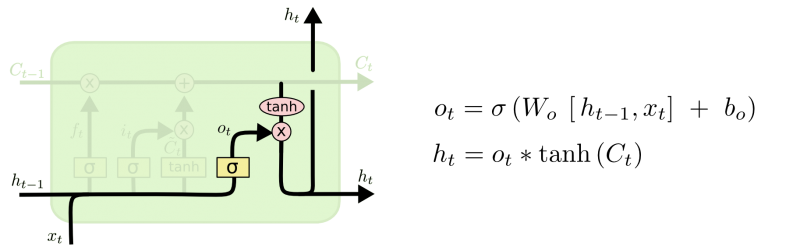
\includegraphics[scale=0.4]{lstm_module_output.png}
\caption{Output của một module}
\end{figure} 
}
\end{frame}

\section{Kết quả thực nghiệm}
\subsection{Dữ liệu thực nghiệm}
\begin{frame}{Dữ liệu thực nghiệm}
\begin{itemize}
\item Bộ dữ liệu IMDB
\item 50000 đánh giá của các bộ phim
\begin{itemize}
\item 25000 đánh giá cho tập training
\item 25000 đánh giá cho tập test 
\end{itemize}
\item Hai nhãn
\begin{itemize}
\item Tích cực
\item Tiêu cực
\end{itemize}
\end{itemize}
\end{frame}

\subsection{Kết quả}
\begin{frame}{LSTM}
\begin{itemize}
\item Mô hình: $INPUT \rightarrow WordEmbedding \rightarrow LSTM \rightarrow sigmoid \rightarrow output$
\begin{itemize}
\item Đầu vào là câu gồm 500 từ
\item Chuyển thành 500 vector số thực 32 chiều.
\item 100 module cuối cùng của LSTM đưa ra output 
\item Output của 100 module đưa vào neuron sigmoid
\end{itemize}
\item Môi trường thực nghiệm:
\begin{itemize}
\item Hệ điều hành Unbutun 16.04 64 bit
\item Intel Core i5-4210U CPU 1.70GHz $\times$ 4
\end{itemize}
\item Kết quả: Độ chính xác 84.97\%
\\[0.2cm]{\small
Epoch 1/3\\
25000/25000 [======] - 498s - loss: 0.5891 - acc: 0.6910\\
Epoch 2/3\\
25000/25000 [======] - 472s - loss: 0.3168 - acc: 0.8696\\   
Epoch 3/3\\
25000/25000 [======] - 466s - loss: 0.2502 - acc: 0.9026\\[0.2cm]
Accuracy: 84.97\% \\
}
\end{itemize}
\end{frame}


\end{document}
